% Foliensatz: "AFu-Kurs nach DJ4UF" von DK0TU, Amateurfunkgruppe der TU Berlin
% Lizenz: CC BY-NC-SA 3.0 de (http://creativecommons.org/licenses/by-nc-sa/3.0/de/)
% Autoren: Sebastian Lange <dl7bst@dk0tu.de>, Lars Weiler <dc4lw@darc.de>

\documentclass[aspectratio=169]{beamer}

\usepackage[ngerman]{babel} % deutsche Worttrennung etc.
\usepackage[utf8]{inputenc} % UTF8 Text

\usepackage[super, comma, numbers, square, sort]{natbib}

\usepackage{hyperref}       % Hyperref Package für bessere Referenzen (todo)
\hypersetup{
	colorlinks=false,       %   false: boxed links; true: colored links
    %linkcolor=white,       %   color of internal links (change box color with linkbordercolor)
    citecolor=red,          %   color of links to bibliography
    filecolor=white,        %   color of file links
    urlcolor=blue           %   color of external links
}

\usepackage{multirow}
\usepackage{wasysym}  % Math Symbols like \permil
%\usepackage{colortbl}
%\usepackage{subscript}
%\usepackage{caption}
%\usepackage{setspace}
%\usepackage{xcolor}        % benutze CodeListe

% Footnote
%\usepackage{hanging}
%
%\setbeamertemplate{footnote}{%
%  \hangpara{2em}{1}%
%  \makebox[2em][l]{\insertfootnotemark}\footnotesize\insertfootnotetext\par%
%}


%\usepackage{pgf}
%\usepackage{tikz}
%\usetikzlibrary{arrows,automata}
%\usetikzlibrary{positioning}
%
%\tikzset{
%    state/.style={
%           rectangle,
%           rounded corners,
%           draw=black, very thick,
%           minimum height=2em,
%           minimum width=2pt,
%           inner sep=2pt,
%           text centered,
%           },
%}

%\usepackage{listings}
%\lstset{basicstyle=\small, numberstyle=\tiny, extendedchars=true, numbers=left, numbersep=5pt}
%\lstset{showtabs=false, showspaces=false, showstringspaces=false}
%%\lstset{backgroundcolor=\color{white!75!lightgray}, , frame=single}
%%\lstset{backgroundcolor=\color{white}}
%%\lstset{backgroundcolor=none}
%\lstset{keywordstyle=\color{blue!50!gray},  identifierstyle=\color{black}}
%\lstset{commentstyle=\color{green!50!gray}, stringstyle=\color{red!50!gray}}
%\lstset{language=C, fontadjust=true, tabsize=2, breaklines=true}
%\lstset{backgroundcolor=\color{white!75!lightgray}, caption=\lstname, frame=single}
%\lstset{emphstyle=\color{black}\fbox}
%
%% Keine "Listing:"-Caption
%\captionsetup{labelformat=empty,labelsep=none}
%
%% für mathematische Umgebungen
%\usepackage{amsmath,amsfonts,amssymb}
%
%\lstdefinestyle{Bash}{
%language=Bash,
%frame=single,
%rulecolor=\color{black},
%backgroundcolor=\color{gray!50},
%keywordstyle=\color{black},
%identifierstyle=,
%commentstyle=\color{black},
%stringstyle=\color{magenta!65!white},
%showstringspaces=false,
%basicstyle=\footnotesize\ttfamily\color{black},
%numbers=none,
%breaklines=true,
%captionpos=b
%}

%\usepackage{listings}
%
%\lstdefinestyle{basic}{
%    captionpos=t,%
%    basicstyle=\footnotesize\ttfamily,%
%    numberstyle=\tiny,%
%    numbers=left,%
%    stepnumber=1,%
%    frame=single,%
%    showspaces=false,%
%    showstringspaces=false,%
%    showtabs=false,%
%    %
%    keywordstyle=\color{blue},%
%    identifierstyle=,%
%    commentstyle=\color{gray},%
%    stringstyle=\color{magenta}%
%}



% fließende Boxen haben keinen Abstand
%\fboxsep0mm

% inkludiere Creative Commons Helper
%%%%%%%%%%%%%%%%%%%%%%%%%%%%%%%%%%%%%%%%%%%%%%%%%%%%%%%%%%%%%%%%
%% ccBeamer 0.1, 2007-07-02                                   %%
%% Written by Sebastian Pipping <webmaster@hartwork.org>      %%
%% ---------------------------------------------------------- %%
%% Licensed under Creative Commons Attribution-ShareAlike 3.0 %%
%% http://creativecommons.org/licenses/by-sa/3.0/             %%
%%%%%%%%%%%%%%%%%%%%%%%%%%%%%%%%%%%%%%%%%%%%%%%%%%%%%%%%%%%%%%%%


%% Images
\newcommand{\CcImageBy}[1]{%
	
\includegraphics[scale=#1]{texdata/creative_commons/cc_by_30.pdf}%
}
\newcommand{\CcImageCc}[1]{%
	
\includegraphics[scale=#1]{texdata/creative_commons/cc_cc_30.pdf}%
}
\newcommand{\CcImageDevNations}[1]{%
	
\includegraphics[scale=#1]{texdata/creative_commons/cc_dev_nations_30.pdf}%
}
\newcommand{\CcImageNc}[1]{%
	
\includegraphics[scale=#1]{texdata/creative_commons/cc_nc_30.pdf}%
}
\newcommand{\CcImageNd}[1]{%
	
\includegraphics[scale=#1]{texdata/creative_commons/cc_nd_30.pdf}%
}
\newcommand{\CcImagePd}[1]{%
	
\includegraphics[scale=#1]{texdata/creative_commons/cc_pd_30.pdf}%
}
\newcommand{\CcImageSa}[1]{%
	
\includegraphics[scale=#1]{texdata/creative_commons/cc_sa_30.pdf}%
}
\newcommand{\CcImageSampling}[1]{%
	
\includegraphics[scale=#1]{texdata/creative_commons/cc_sampling_30.pdf}%
}
\newcommand{\CcImageSamplingPlus}[1]{%
	
\includegraphics[scale=#1]{texdata/creative_commons/cc_sampling_plus_30.pdf}%
}


%% Groups
\newcommand{\CcGroupBy}[2]{% zoom, gap
	\CcImageCc{#1}\hspace*{#2}\CcImageBy{#1}%
}
\newcommand{\CcGroupByNc}[2]{% zoom, gap
	\CcImageCc{#1}\hspace*{#2}\CcImageBy{#1}\hspace*{#2}\CcImageNc{#1}%
}
\newcommand{\CcGroupByNcNd}[2]{% zoom, gap
	\CcImageCc{#1}\hspace*{#2}\CcImageBy{#1}\hspace*{#2}\CcImageNc{#1}\hspace*{#2}\CcImageNd{#1}%
}
\newcommand{\CcGroupByNcSa}[2]{% zoom, gap
	\CcImageCc{#1}\hspace*{#2}\CcImageBy{#1}\hspace*{#2}\CcImageNc{#1}\hspace*{#2}\CcImageSa{#1}%
}
\newcommand{\CcGroupByNd}[2]{% zoom, gap
	\CcImageCc{#1}\hspace*{#2}\CcImageBy{#1}\hspace*{#2}\CcImageNd{#1}%
}
\newcommand{\CcGroupBySa}[2]{% zoom, gap
	\CcImageCc{#1}\hspace*{#2}\CcImageBy{#1}\hspace*{#2}\CcImageSa{#1}%
}
\newcommand{\CcGroupDevNations}[2]{% zoom, gap
	\CcImageCc{#1}\hspace*{#2}\CcImageDevNations{#1}%
}
\newcommand{\CcGroupNcSampling}[2]{% zoom, gap
	\CcImageCc{#1}\hspace*{#2}\CcImageNc{#1}\hspace*{#2}\CcImageSampling{#1}%
}
\newcommand{\CcGroupPd}[1]{% zoom
	\CcImagePd{#1}%
}
\newcommand{\CcGroupSampling}[1]{% zoom
	\CcImageSampling{#1}%
}
\newcommand{\CcGroupSamplingPlus}[1]{% zoom
	\CcImageSamplingPlus{#1}%
}


%% Text
\newcommand{\CcLongnameBy}{Attribution}
\newcommand{\CcLongnameByNc}{Attribution-NonCommercial}
\newcommand{\CcLongnameByNcNd}{Attribution-NoDerivs}
\newcommand{\CcLongnameByNcSa}{Attribution-NonCommercial-ShareAlike}
\newcommand{\CcLongnameByNd}{Attribution-NoDerivs}
\newcommand{\CcLongnameBySa}{Attribution-ShareAlike}

\newcommand{\CcNote}[1]{% longname
	This work is licensed under the \textit{Creative Commons #1 3.0 License}.%
}


% generelles Thema auswählen
\usetheme{Goettingen} %Berlin spart ohne Sidebar allerdings angenehm Platz
% AnnArbor | Antibes | Bergen | Berkeley | Berlin | Boadilla | boxes | CambridgeUS | Copenhagen | Darmstadt | default | Dresden | Frankfurt | Goettingen | Hannover | Ilmenau | JuanLesPins | Luebeck | Madrid | Malmoe | Marburg | Montpellier | PaloAlto | Pittsburgh | Rochester | Singapore | Szeged | Warsaw

% Farben wählen
\usecolortheme{beetle}
% beaver | beetle | crane | default | dolphin | dove | fly | lily | orchid | rose | seagull | seahorse | sidebartab | structure | whale | wolverine

% Setze alle Farben auf Grau und Weiß
%\definecolor{craneorange}{RGB}{64,64,64}
%\definecolor{craneblue}{RGB}{255,255,255}

% Schriftart wählen
\usefonttheme{default}
% default | professionalfonts | serif | structurebold | structureitalicserif | structuresmallcapsserif

% Innere Themen(Kopf-, Fuß-, Sidebar usw)
%\useinnertheme{default}
\useinnertheme{circles}
% default | inmargin | rectangles | rounded | circles

% Äußere Themen (Anordnung der inneren, grenzen der Folien etc.)
\useoutertheme{infolines}
% default | infolines | miniframes | shadow | sidebar | smoothbars | smoothtree | split | tree

% Deaktiviere Navigations-Symbole ({} -> leer)
\setbeamertemplate{navigation symbols}{}
%\setbeamertemplate{navigation symbols}{\large \ifnum \insertframenumber <10 0\fi\insertframenumber/\inserttotalframenumber\vspace*{0.2ex}}

% Zeige ein Hintergrundbild
\setbeamertemplate{background canvas}{
        \hspace*{-2.0cm}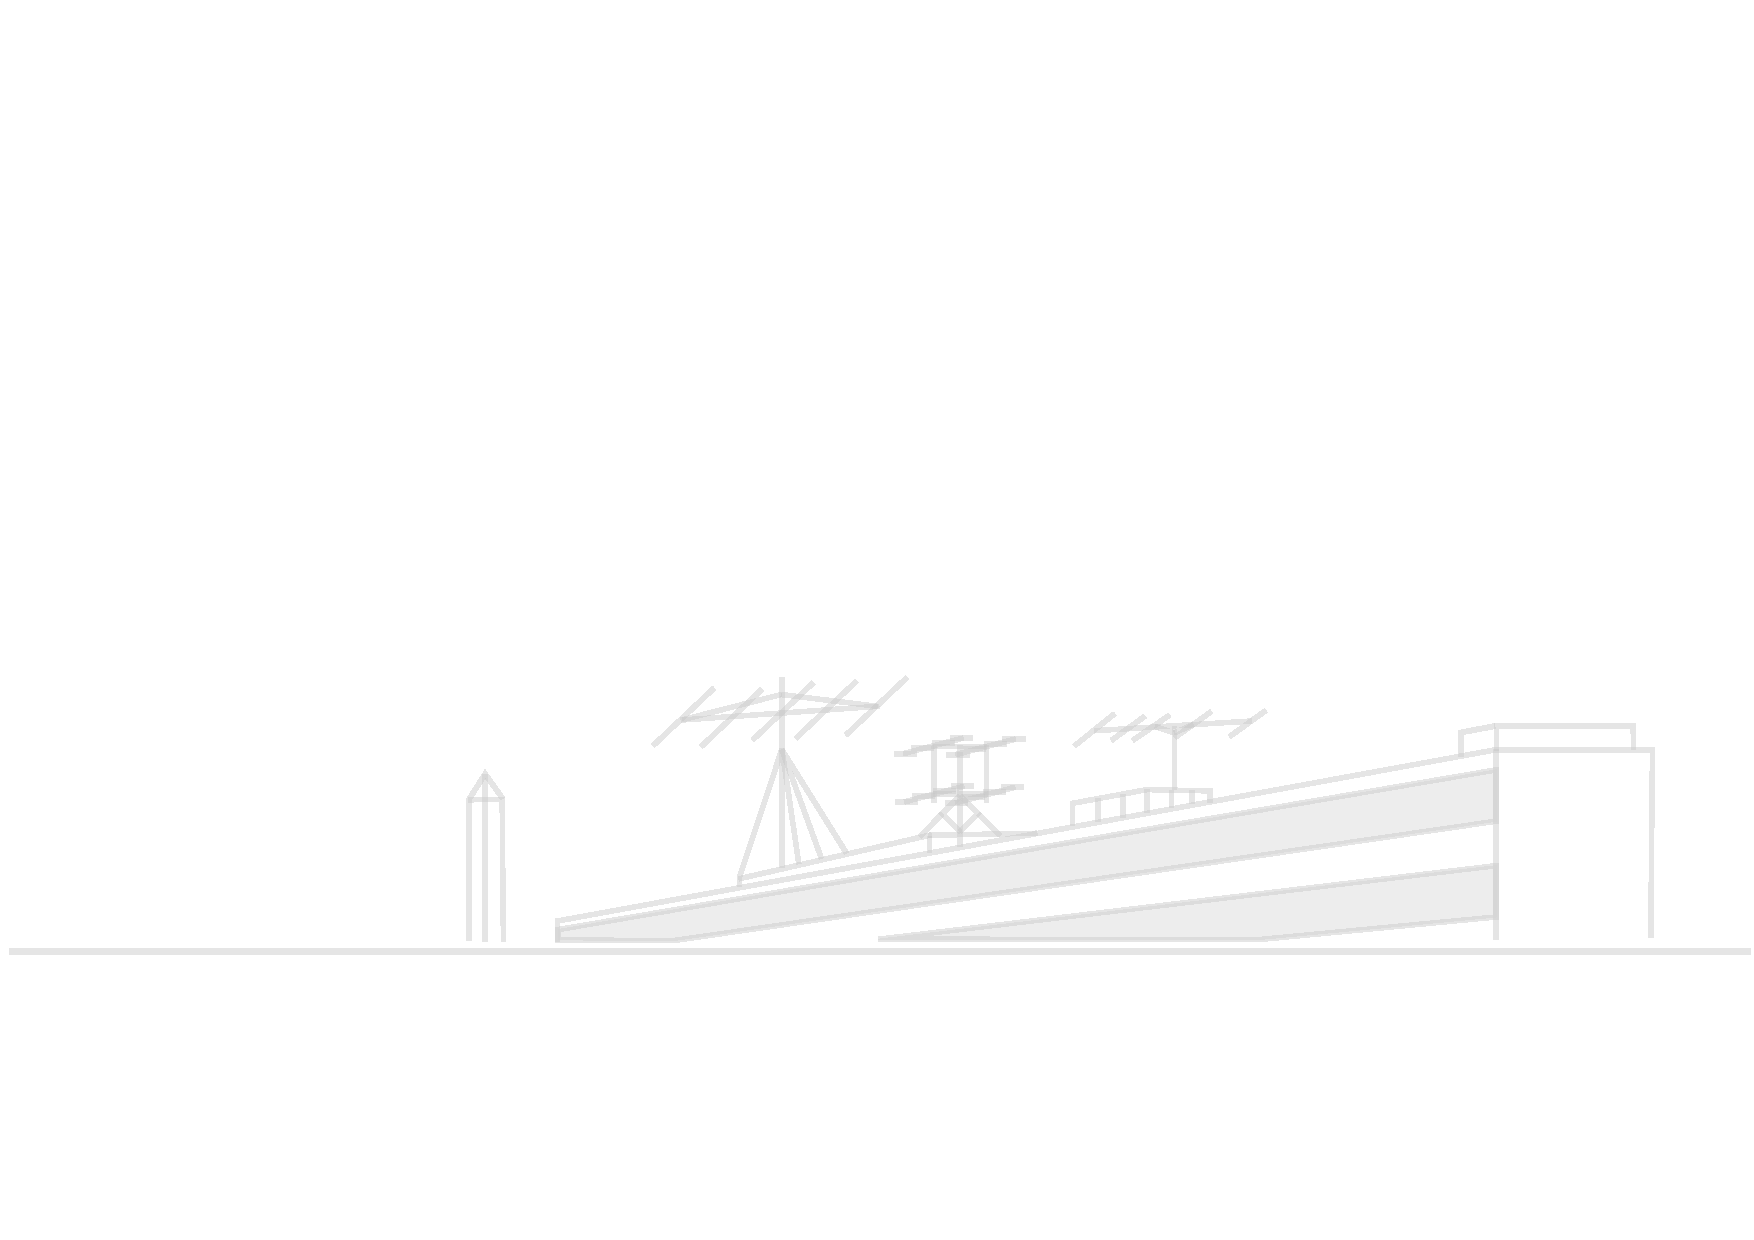
\includegraphics[width=17.8cm]{texdata/dk0tu_rooftop_background.pdf}
}

% Foliennummer einfügen
\setbeamertemplate{footline}[frame number]
%\setbeamertemplate{footline}{}

% Ändere das Zeichen vor jedem item
%\setbeamertemplate{itemize item}{\color{craneorange}$\blacktriangleright$}
%\setbeamertemplate{itemize subitem}{\color{craneorange}$\triangleright$}
%\setbeamertemplate{itemize subsubitem}{\color{craneorange}$\blacktriangleright$}

% Ändert die Blöcke 
\setbeamertemplate{blocks}[rounded][shadow=true]
% default | rounded [shadow=true|false]

%
% Eigene Kommandos
%

% Hack to get natbib and beamer working together. "The beamer user guide suggests
% that only the manual bibliography entry approach is supported"
% on some system it works out of the box, sometimes you need the hack :-(
% so check it --dl7bst
\ifdefined\newblock
    \relax
\else
    \newcommand{\newblock}{}
\fi

% \includedia command to generate png out of a dia file
% NEEDS installed dia and pdflatex option --shell-escape
\newcommand{\includedia}[1]{
    \immediate\write18{/usr/bin/dia #1.dia -e #1_diatmp.png -t png}
}

% RICHIG GROSSER FONT!
\newfont{\bigfont}{cmr10 at 144pt}
\newfont{\smallfont}{cmr10 at 8pt}

% Römische Ziffern
\makeatletter
\newcommand{\rmnum}[1]{\romannumeral #1}
\newcommand{\Rmnum}[1]{\expandafter\@slowromancap\romannumeral #1@}
\makeatother

% Schwarze Überschrift
%\setbeamercolor{frametitle}{fg=black}
%\setbeamercolor{title}{fg=black}

% Item- und Box-Farben
\definecolor{deepBlue}{HTML}{000066}
\setbeamercolor{itemize item}{fg=deepBlue}
\setbeamercolor{itemize subitem}{fg=deepBlue}
\setbeamercolor{description item}{fg=deepBlue}
\setbeamercolor{block title}{fg=deepBlue!100, bg=blue!15}
\setbeamercolor{block body}{fg=black, bg=blue!5}
\setbeamercolor{block title alerted}{fg=deepBlue, bg=red!75}
\setbeamercolor{block body alerted}{fg=black, bg=red!15}
\setbeamercolor*{block title example}{fg=blue!50, bg=blue!10}
\setbeamercolor*{block body example}{fg= blue, bg=blue!5}

%\setbeamercolor{section in head/foot}{parent=palette primary}
%\setbeamercolor{subsection in head/foot}{parent=palette secondary}
%\setbeamercolor{sidebar}{fg=darkblue,bg=yellow!90!orange}
%\setbeamercolor{title in sidebar}{fg=darkblue}
%\setbeamercolor{author in sidebar}{fg=darkblue}
%\setbeamercolor{section in sidebar}{fg=darkblue!10!black}
%\setbeamercolor{subsection in sidebar}{fg=darkblue!50!black}

% Titlepage Infos
\title{AFu-Kurs nach DJ4UF}
\author[DKØTU]{DKØTU\\ \footnotesize{Amateurfunkgruppe der TU Berlin}}
\institute[DKØTU]{\url{http://www.dk0tu.de} }

% PDF-Eigenschaften
\subject{DK0TU-Amateurfunkkurs nach DJ4UF}
\keywords{Amateurfunk Kurs HAM Radio Course CC-BY-NC-SA OpenSource TU Berlin DK0TU}

\subtitle{Technik Klasse E 08: \\
          Elektromagnetisches Feld \\[2em]}
\date{Stand 03.12.2015}
 \begin{document}

\begin{frame}
    \titlepage
    \vfill
    \begin{center}
        \ccbyncsaeu\\
        {\tiny This work is licensed under the \em{Creative Commons Attribution-NonCommercial-ShareAlike 3.0 License}.}\\[0.5ex]
         \tiny Amateurfunkgruppe der Technische Universität Berlin (AfuTUB), DKØTU
         %\includegraphics[scale=0.5]{img/DK0TU_Logo.pdf}
    \end{center}
\end{frame}


%fixme Referenzen/Fußnoten-Systematik vereinheitlichen

\section*{Elektrisches Feld}
\begin{frame}
\frametitle{Das elektrische Feld}
	\begin{center}
        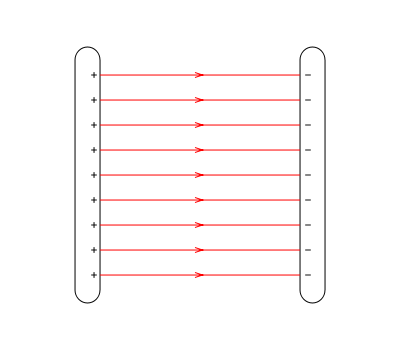
\includegraphics[width=\textwidth,height=.6\textheight,keepaspectratio]{e08/PlattenkondensatorFeld.png}\\
        {\scriptsize Abb. 1: elektrisches Feld zwischen zwei leitenden Platten\\
         (CC-BY 3.0 \url{https://de.wikipedia.org/wiki/Benutzer:Wfstb})}
		\begin{itemize}
			\item wird durch Spannung erzeugt
			\item ist homogen zwischen zwei parallelen Platten
		\end{itemize}
	\end{center}
\end{frame}

\begin{frame}
	\begin{center}
        \begin{block}{Elektrisches Feld}
            \huge$E = \cfrac{U}{d} \text{ in } [\cfrac{V}{m}]$\\
        \end{block}

%		\begin{small}
%		\begin{tabular}{|c|c|c|}
%		\hline
%		\multicolumn{3}{|c|}{\textbf{Berechnen sie das elektrische Feld eines 9V-Blockes}}\\
%		\multicolumn{3}{|c|}{\textbf{mit U = 9V und einem Klemmenabstand von 12,7mm}}\\
%		\hline
%		A & $ 70,87 V/m $    & ??? \\ \hline
%		B & $ 238,19 V/m $   & ??? \\ \hline
%		C & $ 708,66 V/m $   & ??? \\ \hline
%		D & $ 2430,19 V/m $  & ??? \\ \hline
%	\end{tabular}
%	\end{small}		
	\end{center}
\end{frame}

%\begin{frame}
%	\begin{center}
%	\begin{small}
%	\begin{tabular}{|c|c|c|}
%		\hline
%		\multicolumn{3}{|c|}{\textbf{Berechnen sie das elektrische Feld eines 9V-Blockes}}\\
%		\multicolumn{3}{|c|}{\textbf{mit U = 9V und einem Klemmenabstand von 12,7mm}}\\
%		\hline
%		A & $ 70,87 V/m $    & ??? \\ \hline
%		B & $ 238,19 V/m $   & ??? \\ \hline
%		C & $ 708,66 V/m $   & Richtig \\ \hline
%		D & $ 2430,19 V/m $  & ??? \\ \hline
%	\end{tabular}
%	\end{small}		
%	\end{center}
%\end{frame}

% von e06 übernommen
\begin{frame}
    \frametitle{Das magnetische Feld}

    \begin{center}
        \begin{minipage}{0.45\textwidth}
            \begin{center}
                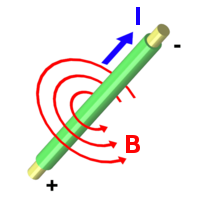
\includegraphics[width=\textwidth,height=.3\textheight,keepaspectratio]{e08/RechteHand.png}\\
                {\scriptsize Abb. 2: magnetisches Feld um einen Leiter\\
                %{\tiny (CC-BY-SA 3.0 \url{https://commons.wikimedia.org/wiki/File:RechteHand.png}}
                }
            \end{center}
        \end{minipage}
        \begin{minipage}{0.45\textwidth}
            \begin{center}
                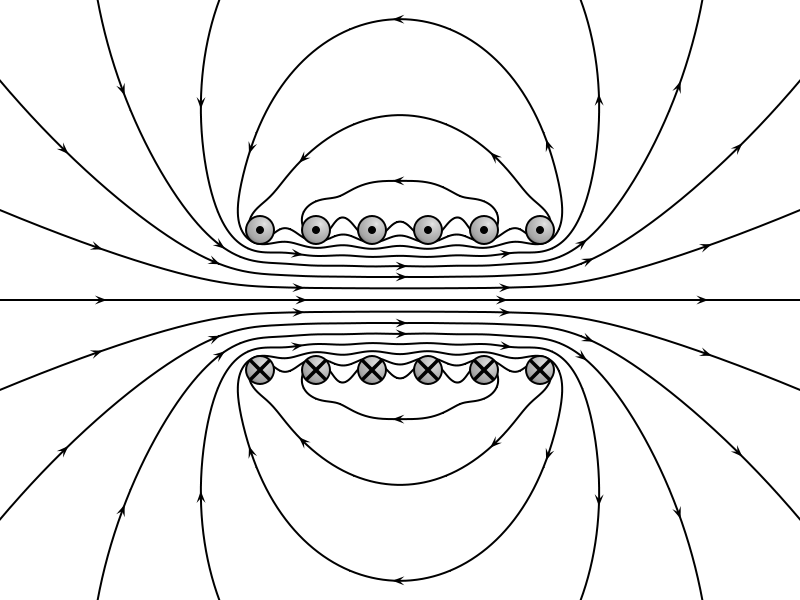
\includegraphics[width=\textwidth,height=.3\textheight,keepaspectratio]{e08/VFPt_cylindrical_coil_real.png}\\
                {\scriptsize Abb. 3: magnetisches Feld in einer Spule\\
                %{\tiny (CC-BY-SA 3.0 \url{https://commons.wikimedia.org/wiki/File:VFPt_cylindrical_coil_real.svg}}
                }
            \end{center}
        \end{minipage}
       
        \bigskip

        \begin{itemize}
            \item um jeden stromdurchflossenen Leiter baut sich ein konzentrisches, magnetisches Feld auf
            \item magnetische Felder summieren sich in einer Spule
            \item magnetische Felder in einer Spule sind homogen
            \item wird mit zunehmendem Strom stärker
            \item nimmt mit zunehmendem Abstand ab
        \end{itemize}

    \end{center}
\end{frame}

\section*{Elektro\-magnetisches Feld}

\begin{frame}
    \frametitle{Das elektromagnetische Feld}

    \begin{center}
        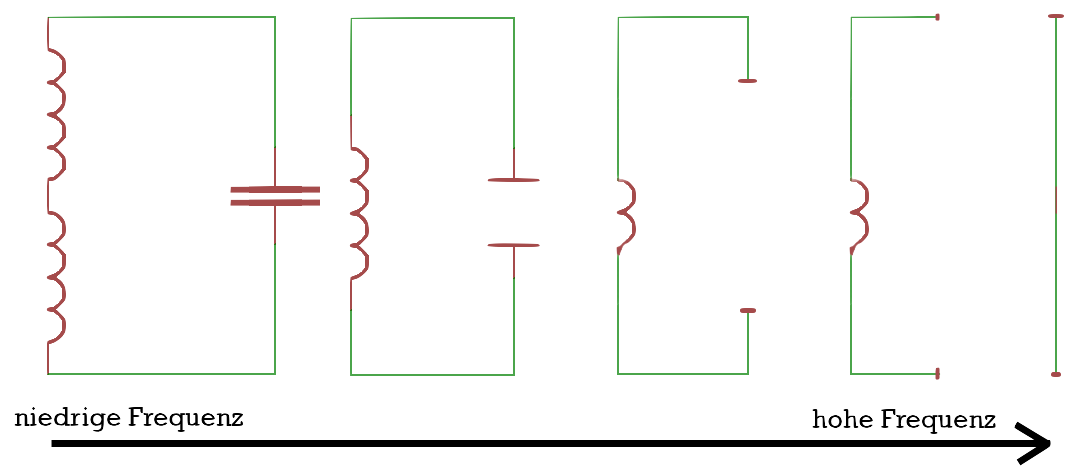
\includegraphics[width=\textwidth,height=.5\textheight,keepaspectratio]{a08/dipol_entstehung.png}\\
        % FIXME Animationen in TeX
        %\animategraphics[loop,width=\textwidth,height=0.5\textheight,keepaspectratio,controls]{3}{e08/Dipolentstehung-}{0}{21}\\
            {\scriptsize Abb. 4: elektromagnetisches Feld
            %{\tiny CC-BY-SA 3.0 \url{https://commons.wikimedia.org/wiki/File:Dipolentstehung.gif}}
            }
    \end{center}

    \begin{itemize}
        \item elektromagnetisches Feld bildet sich durch ein sich änderndes
              elektrisches und ein sich änderndes magnetisches Feld
    	\item zieht man die Kondensatorplatten auseinander und streckt die Spule, erhält man eine Dipolantenne 
    \end{itemize}

\end{frame}

\begin{frame}
    \centering
    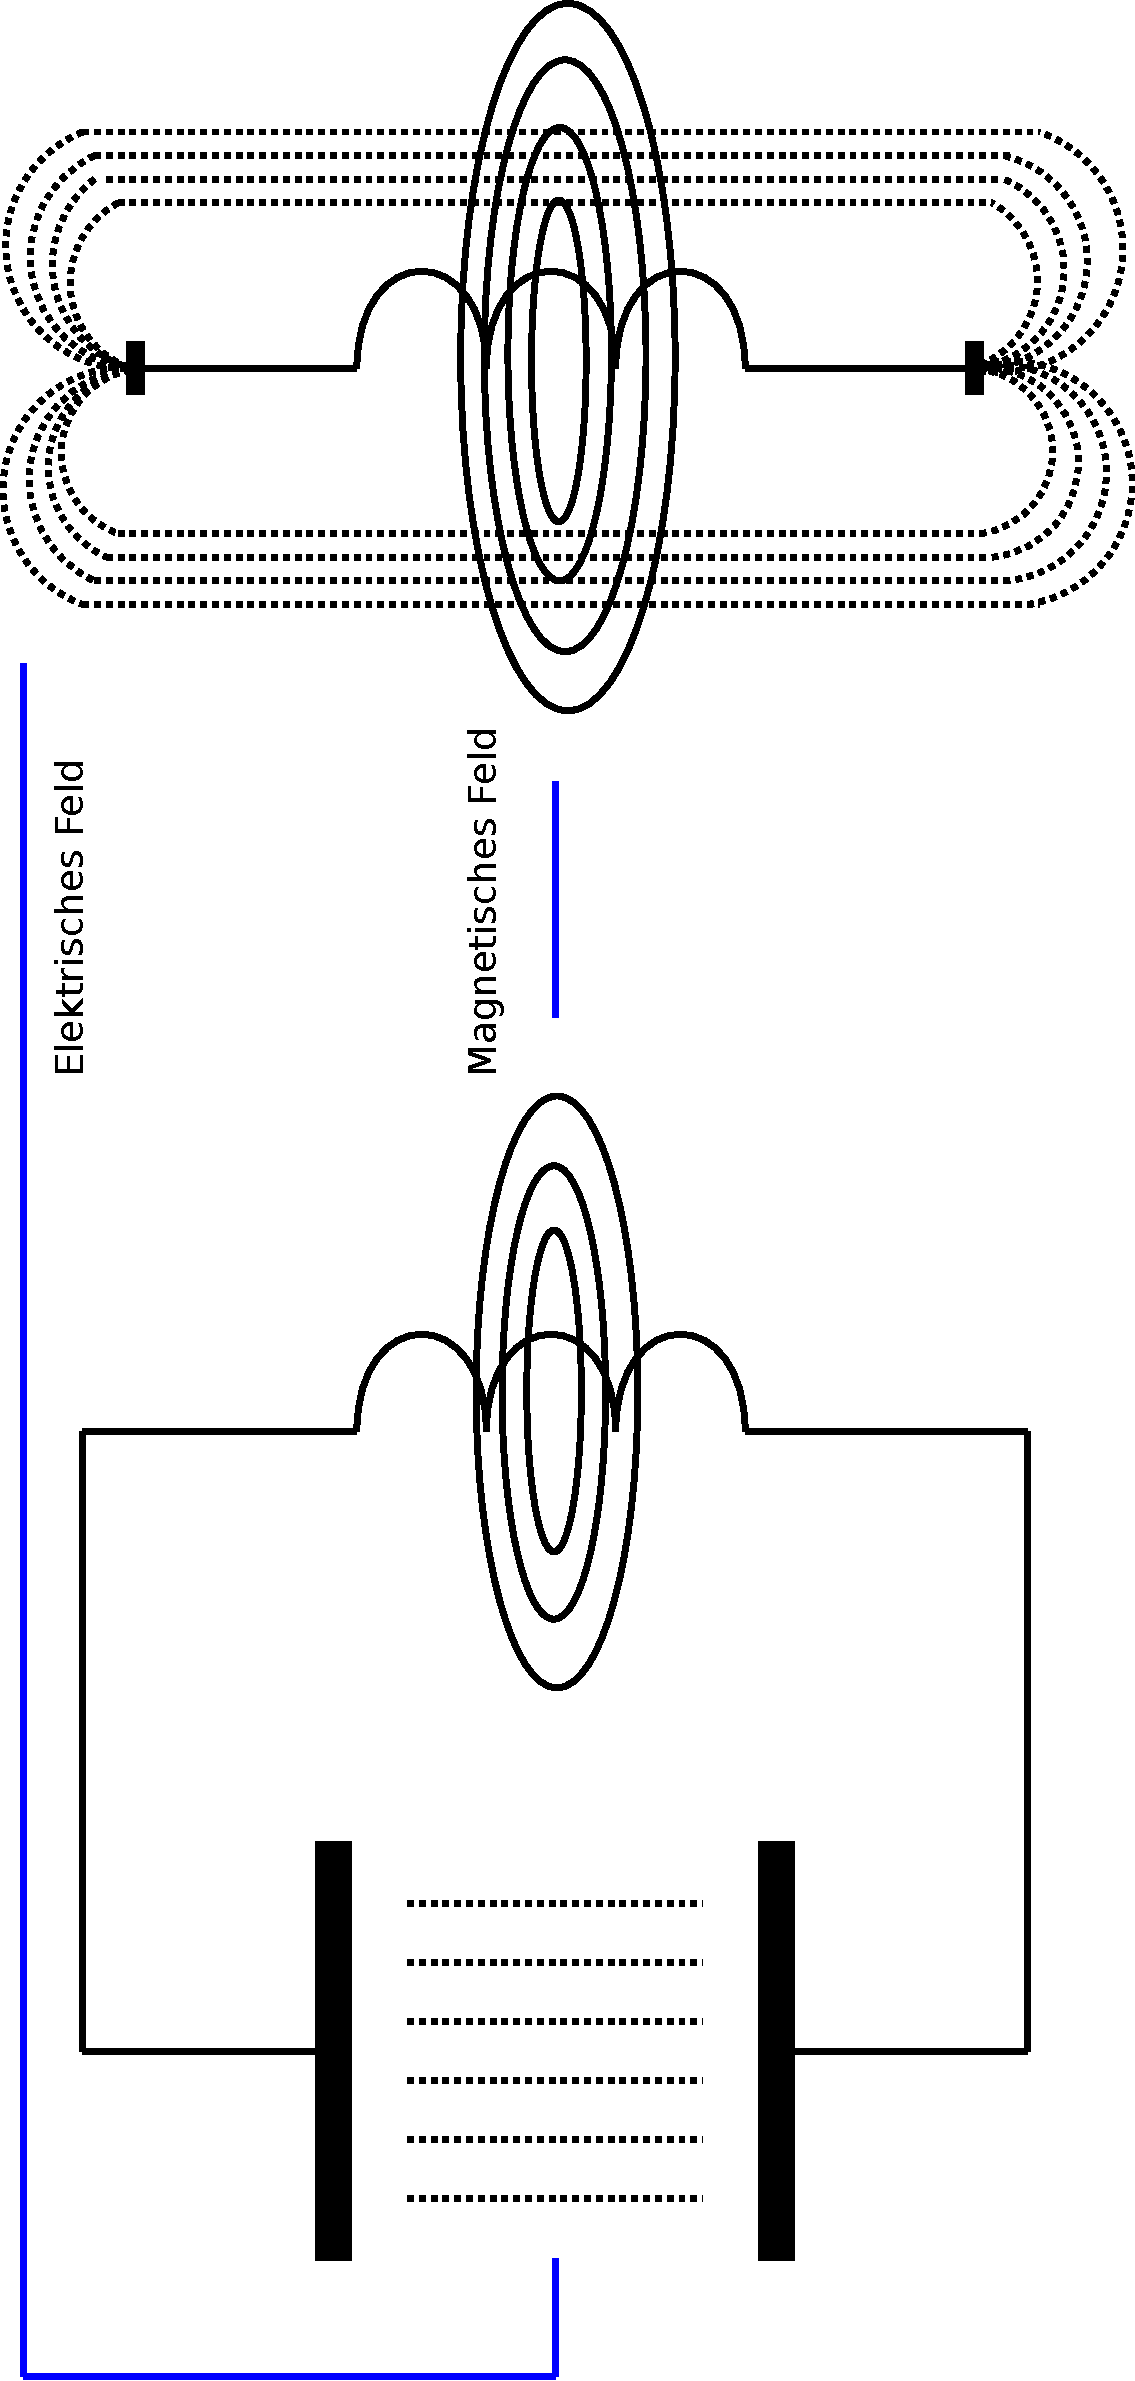
\includegraphics[width=\textwidth,height=1.5\textheight,keepaspectratio,angle=270]{e08/AntSchwingkreis-crop.pdf}\\[1em]
    {\scriptsize Elektromagnetisches Feld im geschlossenen und offenen Schwingreis}
\end{frame}

\section*{Polarisation}

\begin{frame}
    \frametitle{Polarisation}

    \begin{center}
        \begin{minipage}{0.45\textwidth}
            %\animategraphics[loop,width=\textwidth,height=.6\textheight,keepaspectratio,controls]{8}{e08/Dipole_xmting_antenna_animation_4_408x318x150ms-}{0}{7}
            \only<1>{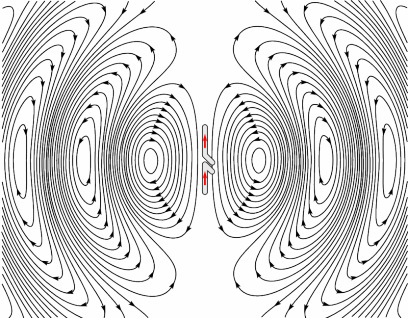
\includegraphics[width=\textwidth,height=.6\textheight,keepaspectratio]{e08/Dipole_xmting_antenna_animation_4_408x318x150ms-0.png}\\}
            \only<2>{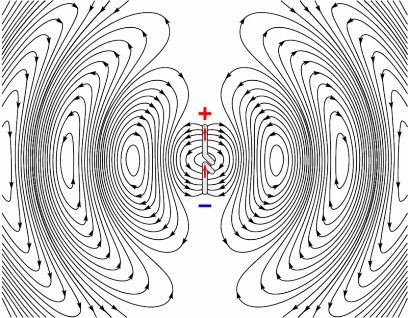
\includegraphics[width=\textwidth,height=.6\textheight,keepaspectratio]{e08/Dipole_xmting_antenna_animation_4_408x318x150ms-1.png}\\}
            \only<3>{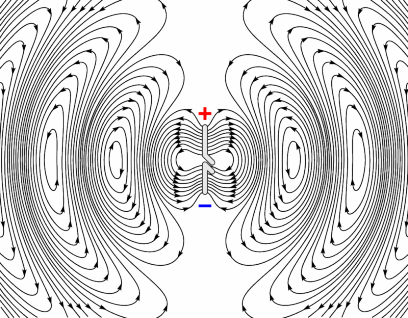
\includegraphics[width=\textwidth,height=.6\textheight,keepaspectratio]{e08/Dipole_xmting_antenna_animation_4_408x318x150ms-2.png}\\}
            \only<4>{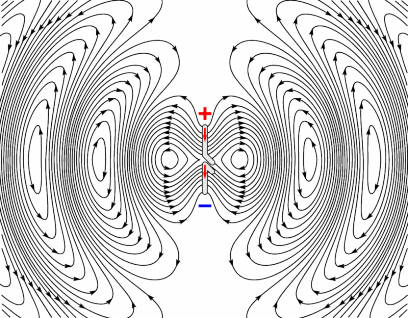
\includegraphics[width=\textwidth,height=.6\textheight,keepaspectratio]{e08/Dipole_xmting_antenna_animation_4_408x318x150ms-3.png}\\}
            \only<5>{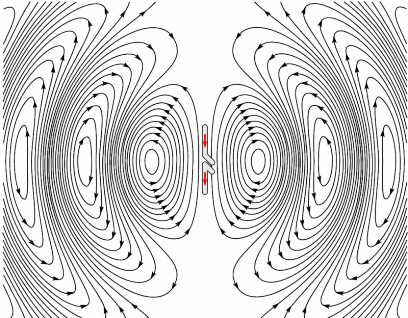
\includegraphics[width=\textwidth,height=.6\textheight,keepaspectratio]{e08/Dipole_xmting_antenna_animation_4_408x318x150ms-4.png}\\}
            \only<6>{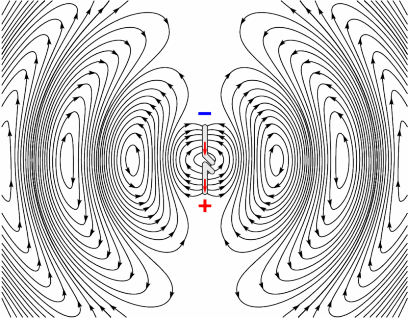
\includegraphics[width=\textwidth,height=.6\textheight,keepaspectratio]{e08/Dipole_xmting_antenna_animation_4_408x318x150ms-5.png}\\}
            \only<7>{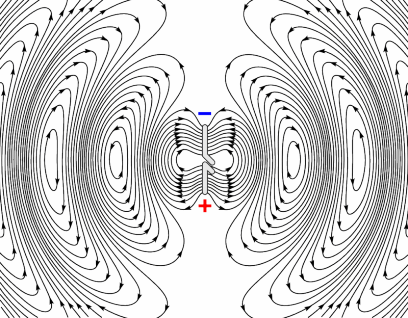
\includegraphics[width=\textwidth,height=.6\textheight,keepaspectratio]{e08/Dipole_xmting_antenna_animation_4_408x318x150ms-6.png}\\}
            \only<8>{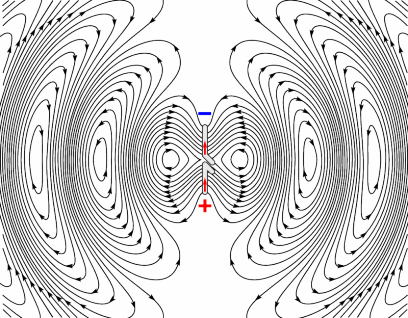
\includegraphics[width=\textwidth,height=.6\textheight,keepaspectratio]{e08/Dipole_xmting_antenna_animation_4_408x318x150ms-7.png}\\}
                {\scriptsize Abb. 4: elektromagnetisches Feld einer Antenne}
                %{\tiny (CC0) \url{https://de.wikipedia.org/wiki/Antennentechnik/media/File:Dipole_xmting_antenna_animation_4_408x318x150ms.gif}}}
	    \end{minipage}
        \begin{minipage}{0.45\textwidth}
            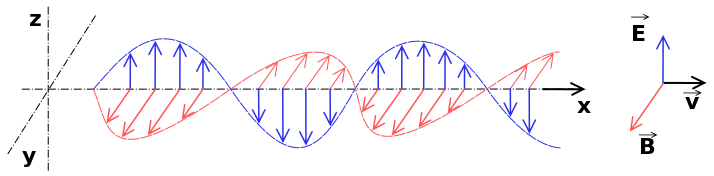
\includegraphics[width=\textwidth,height=.8\textheight,keepaspectratio]{e08/Onde_electromagnetique.png}\\
                {\scriptsize Abb. 5: Polarisation einer Antenne}
                %{\tiny CC-BY-SA 3.0 \url{https://de.wikipedia.org/wiki/Antennentechnik/media/File:Onde_electromagnetique.svg}}}
        \end{minipage}\\[1.5em]

	    \begin{itemize}
	    	\item E-Feld bestimmt die Richtung der Polarisation 
	    	\item magnetisches Feld ist um $90^\circ$ gedreht
	    \end{itemize}
    
    \end{center}

\end{frame}

\section*{Wellenlänge}

\begin{frame}
    \frametitle{Wellenlänge}

    \begin{center}
        \begin{block}{Wellenlänge $\lambda$}
            \begin{center}
                {\Huge$ \lambda [m] = \cfrac{c}{f [Hz]} \Rightarrow
                c = f \cdot \lambda $} \\[1em]
                mit $c$: Lichtgeschwindigkeit $299\,792\,458 \frac{m}{s} \approx
                300\cdot10^6\frac{m}{s}$
            \end{center}
        \end{block}

	    \begin{normalsize}		
	        \begin{itemize}
		        \item elektromagnetische Wellen breiten sich im Freiraum fast mit Lichtgeschwindigkeit aus
		        \item Beispiel: in einer Sekunde bewegt sich eine elektromagnetische Welle mehr als sieben mal um die Erde
	        \end{itemize}
	    \end{normalsize}
    \end{center}
\end{frame}

\begin{frame}
	\begin{center}
	    \begin{Large}
	        \begin{tabular}{|l|l|l|}
	        	\hline
                Frequenz & Wellenlänge & Abkürzung\\
	        	\hline \hline
                3 - 30 kHz     & $10^{4}m$    & VLF \\ \hline
                \textbf{30 - 300 kHz}   & \textbf{$10^{3}m$}      & \textbf{LF}  \\ \hline
                \textbf{300 - 3000 kHz} & \textbf{$10^{2}m$}     & \textbf{MF}  \\ \hline
                \textbf{3 - 30 MHz}     & \textbf{$10^{1}m$}      & \textbf{HF}  \\ \hline
                \textbf{30 - 300 MHz}   & \textbf{$10^{0}m$}          & \textbf{VHF} \\ \hline
                \textbf{300 - 3000 MHz} & \textbf{$10^{-1}m$}      & \textbf{UHF} \\ \hline
                \textbf{3 - 30 GHz}     & \textbf{$10^{-2}m$}     & \textbf{SHF} \\ \hline
                30 - 300 GHz   & $10^{-3}m$     & EHF \\ \hline
                300 - 3000 GHz & $10^{-4}m$ & " " \\ \hline
            \end{tabular}\\[1em]
            {\scriptsize Tabelle 1: Wellenbereiche (fett: Bereiche des Amateurfunks)}
        \end{Large}		
	\end{center}
\end{frame}

%\section*{Übung}
%
%\begin{frame}
%	\begin{center}
%        \begin{tabular}{l||p{.8\textwidth}}\hline
%            \textbf{TB403} & \textbf{Wenn Strom durch einen gestreckten Leiter fließt, entsteht ein \ldots} \\\hline\hline
%            A & elektrisches Feld aus konzentrischen Kreisen um den Leiter. \\ \hline
%            B \only<2>\checkmark & Magnetfeld aus konzentrischen Kreisen um den Leiter. \\ \hline
%            C & homogenes Magnetfeld um den Leiter. \\ \hline
%            D & homogenes elektrisches Feld um den Leiter. \\ \hline
%	    \end{tabular}
%	\end{center}
%\end{frame}
%
%\begin{frame}
%	\begin{center}
%        \begin{tabular}{l||p{.8\textwidth}}\hline
%           \textbf{TB301} & \textbf{Welche Einheit wird für die elektrische Feldstärke verwendet?} \\\hline\hline
%           A & Watt pro Quadratmeter ($W/m^2$) \\ \hline
%           B & Ampere pro Meter ($A/m$) \\ \hline
%           C & Henry pro Meter ($H/m$) \\ \hline
%           D \only<2>\checkmark & Volt pro Meter ($V/m$) \\ \hline
%	    \end{tabular}
%    \end{center}
%\end{frame}
%
%\begin{frame}
%	\begin{center}
%        \begin{tabular}{l||p{.8\textwidth}}\hline
%           \textbf{TB401} & \textbf{Welche Einheit wird für die magnetische Feldstärke verwendet?} \\\hline\hline
%           A & Watt pro Quadratmeter ($W/m^2$) \\ \hline
%           B \only<2>\checkmark & Ampere pro Meter ($A/m$) \\ \hline
%           C & Henry pro Meter ($H/m$) \\ \hline
%           D & Volt pro Meter ($V/m$) \\ \hline
%	    \end{tabular}
%	\end{center}
%\end{frame}
%
%\begin{frame}
%    \begin{center}
%        \begin{tabular}{l||p{.8\textwidth}}\hline
%            \textbf{TB501} & \textbf{Wodurch entsteht ein elektromagnetisches Feld?
%                                     Ein elektromagnetisches Feld entsteht,} \\\hline\hline
%            A \only<2>\checkmark & wenn ein zeitlich schnell veränderlicher
%                                   Strom durch einen elektrischen Leiter
%                                   fließt, dessen Länge mindestens 1/100 der Wellenlänge ist. \\ \hline
%            B & wenn durch einen elektrischen Leiter, dessen Länge mindestens
%                1/100 der Wellenlänge ist, ein konstanter Strom fließt. \\ \hline
%            C & wenn sich elektrische Ladungen in einem Leiter befinden, dessen
%                Länge mindestens 1/100 der Wellenlänge ist. \\ \hline
%            D & wenn an einem elektrischen Leiter, dessen Länge mindestens
%                1/100 der Wellenlänge ist, eine konstante Spannung angelegt wird. \\ \hline
%	    \end{tabular}
%	\end{center}
%\end{frame}
%
%\begin{frame}
%	\begin{center}
%        \begin{tabular}{l||p{.8\textwidth}}\hline
%            \textbf{TB504} & \textbf{Der Winkel zwischen den elektrischen und magnetischen Feldkomponenten eines elektromagnetischen Feldes beträgt im Fernfeld}\\ \hline\hline
%            A & $45^\circ$. \\ \hline
%            B \only<2>\checkmark & $90^\circ$. \\ \hline
%            C & $180^\circ$. \\ \hline
%            D & $360^\circ$. \\ \hline
%	    \end{tabular}
%	\end{center}
%\end{frame}
%
%\begin{frame}
%	\begin{center}
%        \begin{tabular}{l||p{.8\textwidth}}\hline
%            \textbf{TI201} & \textbf{Die Ausbreitungsgeschwindigkeit freier elektromagnetischer Wellen beträgt etwa \ldots}\\ \hline\hline
%            A & $3\,000\,000\,km/s$. \\ \hline
%            B & $30\,000\,km/s$. \\ \hline
%            C \only<2>\checkmark & $300\,000\,km/s$. \\ \hline
%            D & $3\,000\,km/s$. \\ \hline
%	    \end{tabular}
%    \end{center}
%\end{frame}
%
%\begin{frame}
%	\begin{center}
%        \begin{tabular}{l||p{.8\textwidth}}\hline
%            \textbf{TB602} & \textbf{Welcher Wellenlänge $\lambda$ entspricht die Frequenz 1,84MHz?} \\ \hline\hline
%            A & 16,3m \\ \hline
%            B \only<2>\checkmark & 163m \\ \hline
%            C & 0,613m \\ \hline
%            D & 61,3m \\ \hline
%	    \end{tabular}
%	\end{center}
%\end{frame}
%
%\begin{frame}
%	\begin{center}
%       \begin{tabular}{l||p{.8\textwidth}}\hline
%         \textbf{TB604} & \textbf{Eine Wellenlänge von 2,06m entspricht einer Frequenz von~\ldots} \\ \hline\hline
%           A & 135,754 MHz \\ \hline
%           B & 148,927 MHz \\ \hline
%           C & 150,247 MHz \\ \hline
%           D \only<2>\checkmark & 145,631 MHz \\ \hline
%	    \end{tabular}
%	\end{center}
%\end{frame}
%
%\begin{frame}
%	\begin{center}
%       \begin{tabular}{l||p{.8\textwidth}}\hline
%         \textbf{TB609} & \textbf{Das 70-cm-Band befindet sich im \ldots} \\ \hline\hline
%           A & VHF-Bereich. \\ \hline
%           B \only<2>\checkmark & UHF-Bereich. \\ \hline
%           C & SHF-Bereich. \\ \hline
%           D & EHF-Bereich. \\ \hline
%        \end{tabular}
%	\end{center}
%\end{frame}

\section*{Referenzen}
\begin{frame}
    \frametitle{Referenzen/Links}
    
    \footnotesize
    \begin{itemize}
        \item Moltrecht E 08 : \\
              \url{http://www.darc.de/referate/ajw/ausbildung/darc-online-lehrgang/technik-klasse-e/technik-e08/}      
    \end{itemize}

\end{frame}

% Hier könnte noch eine Kontaktfolie stehen

\end{document}

